\section{方法} 
\label{sec:proposed}

这一章节将对基于 Mean Shift 和机遇分类思想的两种目标跟踪方法进行介绍,其结果将在实验部分给出。

\subsection{目标跟踪的基本框架}

跟踪算法通常同时依赖外观建模和运动信息建模。如图 \ref{fig:tracker_example} 所示,通过利用初始帧的目标外观信息进行建模后,跟踪器具有了目标和背景的辨别能力。在后续帧中,跟踪算法首先通过运动模型,如粒子滤波,粗略地估计目标位置并得到一系列的候选样本,进一步结合外观模型进行目标的精准定位。准确的定位用于更新运动模型和外观模型。因此,两种目标跟踪方法的初始目标位置标定都依赖于手工标定,后续帧中的目标位置则分别通过均值漂移方法和在线分类器得到。

\subsection{基于均值漂移的目标跟踪}

均值漂移 (Mean Shift) 的基本思想是利用概率密度的梯度爬升来寻找局部最优,即 Mean Shift 向量逐步漂移到局部密度最大点并停止,从而达到跟踪目的。

\subsubsection{Mean Shift}

给定 $d$ 维空间中的 $n$ 个样本点 $x_i(i=1, \ldots, n)$,在 $x$ 点的 Mean Shift 向量的基本形式定义为:
\vspace{0.5cm}

\begin{equation}
M_h(x)=\left(\frac{1}{k} \sum_{x_i \in S_h} x_i\right)-x=\frac{1}{k} \sum_{x_i \in S_h}\left(x_i-x\right)
\vspace{0.5cm}
\end{equation}

其中, $S_h$ 是一个半径为 $h$ 的高维球区域, $k$ 表示 $n$ 个样本点中有 $k$ 个点落入区域 $S_h$ 中。直观地, Mean Shift 向量表示区域中 $k$ 个样本点相对于点 $x$ 求偏移向量再平均。该向量指向概率密度梯度的方向。

\begin{figure}[!ht]
	\center
	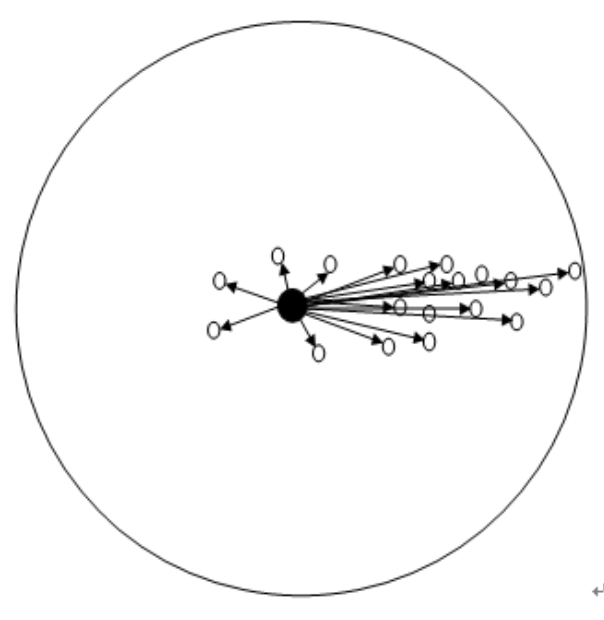
\includegraphics[width=0.65\linewidth]{fig2.png}
	\caption{Mean Shift 示意图}
	\label{fig:meanshift}
\end{figure}

如图 \ref{fig:meanshift} 所示,大圆所圈定的范围即为 $S_h$,小圆代表落入 $S_h$ 区域内的样本点 $x_i \in S_h$,中心的黑色实心圆即为 Mean Shift 的基准点 $x$,箭头表示样本点相对于基准点 $x$ 的偏移向量。可以看出,平均的偏移向量 $M_h(x)$ 会指向样本分量最多的区域,也就是概率密度函数的梯度方向。
\vspace{0.5cm}

\begin{equation}
M_h(x)=\frac{1}{k} \sum_{x_i \in S_h}\left(x_i-x\right)
\vspace{0.5cm}
\end{equation}

\subsubsection{核函数}
为了解决所有样本点对均值平移向量的贡献相同的问题,在 Mean Shift 的基础上引入两个参数,即核函数和权重。核函数的定义为 $x \in R^D,\|x\|^2=x^T x$,若函数 $K(𝑥)$ 存在一个剖面函数: $k:[0, \infty) \rightarrow R$, 即 $K(x)=k\left(\|x\|^2\right)$,并且 $k(𝑟)$ 满足:1)非负的;2)非增的;3)分段连续的,且 $\int_0^{\infty} k(r) d r<\infty$,那么函数 $K(𝑥)$ 就被称为核函数。常用的核函数包括 Epanechikov 核函数、均匀核函数和高斯核函数。本文采用的是 Epanechikov 核函数,即计算空间任意一点到中心位置的欧氏距离。其表达式如下:
\vspace{0.5cm}

\begin{equation}
K_E(\mathbf{x})=\left\{\begin{array}{cr}
c\left(1-\|\mathbf{x}\|^2\right) & \|\mathbf{x}\| \leq 1 \\
0 & \text { otherwise }
\end{array}\right.
\vspace{0.5cm}
\end{equation}

在跟踪问题中,核函数起到了位置加权的作用,即更加相信中心位置像素点的信息。

\subsubsection{均值漂移目标跟踪算法}

基于均值漂移的目标跟踪算法通过分别计算目标区域和候选区域内像素的特征值概率得到关于目标模型和候选模型的描述,然后利用相似函数度量初始帧目标模型和当前帧的候选模版的相似性,选择使相似函数最大的候选模型并得到关于目标模型的 Mean Shift 向量,这个向量正是目标由初始位置向正确位置移动的向量。由于均值漂移算法的快速收敛性,通过不断迭代计算 Mean Shift 向量,算法最终将收敛到目标的真实位置,达到跟踪的目的。流程如下:

(1)目标核函数直方图:
\vspace{1.1cm}

\begin{equation}
\vspace{0.5cm}
\hat{q}_u=C \sum_{i=1}^n \tikzmarknode{x}{\highlight{red}{$k\left(\left\|x_i\right\|^2\right)$}}\tikzmarknode{s}{\highlight{blue}{$\delta\left[b\left(x_i\right)-u\right]$}}.
\end{equation}
\begin{tikzpicture}[overlay,remember picture,>=stealth,nodes={align=left,inner ysep=1pt},<-]
    % For "X"
    \path (x.north) ++ (0,2em) node[anchor=south east,color=red!67] (scalep){\textbf{核函数,中心像素权重更大}};
    \draw [color=red!87](x.north) |- ([xshift=-0.3ex,color=red]scalep.south west);
    % For "S"
    \path (s.south) ++ (0,-1.5em) node[anchor=north west,color=blue!67] (mean){\textbf{统计直方图}};
    \draw [color=blue!57](s.south) |- ([xshift=-0.3ex,color=blue]mean.south east);
\end{tikzpicture}


其中,$C=1 / \sum_{i=1}^n k\left(\left\|x_i\right\|^2\right)$ 为归一化常数,$k$ 表示核函数(在核估计中通常是平滑作用), 目标区域共 $n$ 个像素点 $\left\{x_i\right\}_{i=1, \ldots, r}$,该区域颜色分布离散成 $m$ 级,$b\left(x_i\right)$ 表示像素点 $x_i$ 的量化值。 

(2)在当前帧,计算候选(待跟踪目标)核函数直方图:
\vspace{0.5cm}
\begin{equation}
\hat{p}_u(y)=C_h \sum_{i=1}^{n_h} k\left(\left\|\frac{y-x_i}{h}\right\|^2\right) \delta\left[b\left(x_i\right)-u\right]
\vspace{0.5cm}
\end{equation}

其中,$C_h=1 / \sum_{i=1}^n k\left(\left\|\frac{y-x_i}{h}\right\|^2\right)$,候选目标区域 $\left\{x_i\right\}_{i=1, \ldots, n_h}$ ,该区域的中心位置为 $y$,$h$ 表示核函数 $k$ 的窗宽。其余变量物理意义同上。

(3)计算候选目标与初始目标的相似度:

\vspace{0.5cm}
\begin{equation}
\hat{\rho}(y)=\sum_{u=1}^m \sqrt{\hat{p}_u(y) \hat{q}_u}
\vspace{0.5cm}
\end{equation}

进行 Taylor 展开,将 $\widehat{p}_u(y)$ 代入并化简得到:

\vspace{0.5cm}

\begin{equation}
\hat{\rho}(y) \approx \frac{1}{2} \sum_{u=1}^m \sqrt{\hat{p}_u\left(y_0\right) \hat{q}_u}+\frac{C_h}{2} \sum_{i=1}^{n_h} \mathrm{w}_i k\left(\left\|\frac{y-x_i}{h}\right\|^2\right)
\vspace{0.5cm}
\end{equation}

其中,$\mathrm{w}_i=\sum_{u=1}^m \sqrt{\frac{\hat{q}_u}{\hat{p}_u\left(\hat{y}_0\right)}} \delta\left[b\left(x_i\right)-u\right]$,$y_0$ 是 Mean Shift 迭代的起点位置, 在跟踪中通常是目标在上一帧的位置。由于第一项为常量,因此我们最大化 $\hat{\rho}(y)$ ,本质上寻找新的质心 $y$ 使得候选区域和模板的相似程度最大化。

(4)计算权值 $\{W\}_{i=1,2, \ldots, m}$

(5)利用 Mean Shift 方法求解目标的新位置 $y_1$: 
\vspace{0.5cm}

\begin{equation}
y_1=\frac{\sum_{i=1}^{n_h} x_i w_i g\left(\left\|\frac{y_0-x_i}{h}\right\|^2\right)}{\sum_{i=1}^{n_h} w_i g\left(\left\|\frac{y_0-x_i}{h}\right\|^2\right)}
\vspace{0.5cm}
\end{equation}


代码实现如下:

\vspace{0.3cm}
\lstinputlisting[language=Python,firstline=47,lastline=120]{main.py}

\subsection{基于分类思想的目标跟踪}

如前文所述,基于分类思想的目标跟踪将目标和背景信息同时考虑在内,其基本原理是把跟踪看作分类问题,通过训练分类器来区分背景和目标。具体来讲就是是把目标跟踪看作二分类问题,在线训练作为整体的多个弱分类器用来区分目标和背景。使用 AdaBoost 把作为整体的多个弱分类器合并为一个强的分类器,该分类器用于下一帧的分类,区分像素属于目标还是背景,并得出置信图,并在置信图上利用 Mean Shift 算法找出峰值点也就是目标的位置。在跟踪过程中通过在线训练新的弱分类器并加入到分类器集合里从而在连贯时间上保持更新弱分类器这一整体。

首先需要在第一帧将目标的位置进行手工标注,对于弱分类器而言,所有像素都是潜在的训练数据。为了减少训练时间,本文根据视频训练中目标的大小,将标注目标及其周围的一部分像素(背景)作为训练数据。每个像素都使用一个 11 维的特征向量来描述(由 8 维的 $5\times 5$ 邻域局部方向直方图和 3 维的像素颜色组成),来自目标和背景的像素对应的标签分别为 1 和 -1,即
\vspace{0.3cm}
\begin{equation}
y_i= \begin{cases}+1 & \text { inside }\left(r_j\right) \\ -1 & \text { otherwise }\end{cases}
\vspace{0.3cm}
\end{equation}

其中,$r_j$ 为当前帧的目标位置。

本文使用支持向量机作为弱分类器。对于每一个弱分类器,可以计算其误差率,计算方法为:
\vspace{0.3cm}

\begin{equation}
e r r=\sum_{i=1}^N w_i\left|h_t\left(x_i\right)-y_i\right|
\vspace{0.3cm}
\end{equation}

其中,$w_i$ 是像素的权重,为像素被选择训练的概率。$h_t\left(x_i\right)$ 是像素 $x_i$ 的类别,而 $y_i$ 为其“正确”的类别标签。在初始状态下,所有的像素权重都是相等的,并随着训练过程而不断更新,如果像素被错误分类,则像素权重会随之增加。也就是说,在随后的训练集中,难以分类的像素更有可能被选择。权重的更新公式为:
\vspace{0.3cm}

\begin{equation}
w_i=w_i \exp \left\{\alpha_t\left|h_t\left(x_i\right)-y_i\right|\right\}
\vspace{0.3cm}
\end{equation}


集成学习技术把若干弱分类器组合成一个强的分类器。如本文使用的 AdaBoost 每次在更难的样本上训练一个弱分类器加入到强分类器使得最终的分类器比任何一个弱分类器都好。在跟踪过程中一直更新弱分类器集合,将目标从背景中分离。因此,该方法并不准确的描述目标,而是使用分类器集合来决定一个像素属于目标还是背景,从而可以更好地应对光照、尺寸的变化,目标的变形和遮挡等问题。在集成为强分类器时,需要为每个若分类器赋予一个权重,性能较好的分类器则具有较高的权重,该权重是由弱分类器的误差率决定的:
\vspace{0.3cm}
\begin{equation}
\alpha_t=\frac{1}{2} \log \frac{1-e r r}{e r r}
\vspace{0.3cm}
\end{equation}

其算法流程如算法 \ref{ensemble} 所示。

 \begin{algorithm}
        \caption{Ensemble Tracking}
         \label{ensemble}
        \LinesNumbered
        \KwIn{n video frames $I_1, \cdots, I_n$, Rectangle $r_1$ of object in first frame}
        \KwOut{Rectangles $r_2 , \cdots, r_n$}
        
        Initialization (for frame $I_1$):\\
        Extract $\{x_i\}^N_i=1$ examples with labels $\{y_i\}^N_i=1$\\
        Initialize weights $\{w_i\}^N_i=1$ to be $\frac{1}{N}$\\
        \For{$t = 1 \to T$} 
        {
        (a) Make $\{w_i\}^N_i=1$ a distrubition\\
        (b) Train weak classifier $h_t$\\
        (c) Set $\operatorname{err}=\sum_{i=1}^N w_i\left|h_t\left(\mathbf{x}_{\mathbf{i}}\right)-y_i\right|$\\
        (d) Set weak classifier weight $\alpha_t=\frac{1}{2} \log \frac{1-e r r}{e r r}$\\
        (e) Update example weights $w_i=w_i e^{\left(\alpha_t\left|h_t\left(\mathbf{x}_{\mathbf{i}}\right)-y_i\right|\right)}$\\
        }
        
        The strong classifier is given by $\operatorname{sign}(H(\mathbf{x}))$ where $H(x)=\sum_{t=1}^T \alpha_t h_t(\mathbf{x})$\\
        
         \For{each new frame $I_j$} 
         {
         Extract $\left\{\mathbf{x}_{\mathbf{i}}\right\}_{i=1}^N$ examples\\
         Test the examples using the strong classifier $H(x)$ and create confidence image $L_j$\\
         Run mean-shift on $L_j$ with $r_{j-1}$ as the initial guess. Let $r_j$ be the result of the mean shift algorithm\\
         Define labels $\left\{y_i\right\}_{i=1}^N$ with respect to the new rectangle $r_j$\\
         Remove $K$ oldest weak classifiers\\
         Initialize weights $\left\{w_i\right\}_{i=1}^N$ to be $\frac{1}{N}$\\
         \For(\tcp*[f]{Update weights}){$l=K+1 \to T$}
         {
         (a) Make $\left\{w_i\right\}_{i=1}^N$ a distribution\\
         (b) Choose $h_t(\mathbf{x})$, with minimal error $e r r$, from $\left\{h_{K+1}(\mathbf{x}), \ldots, h_T(\mathbf{x})\right\}$\\
         (c) update $\alpha_t$ and $\left\{w_i\right\}_{i=1}^N$\\
         (d) Remove $h_t(\mathbf{x})$ from $\left\{h_{K+1}(\mathbf{x}), \ldots, h_T(\mathbf{x})\right\}$\\
         }
         
         \For(\tcp*[f]{Add new weak classifiers}){$l=1 \to K$}
         {
         (a) Make $\left\{w_i\right\}_{i=1}^N$ a distribution\\
         (b) Train weak classifier $h_t$\\
         (c) Compute $e r r$ and $\alpha_t$\\
         (d) Update example weights $\left\{w_i\right\}_{i=1}^N$
         }
         
         The updated strong classifier is given by $\operatorname{sign}(H(\mathbf{x}))$ where $H(x)=\sum_{t=1}^T \alpha_t h_t(\mathbf{x})$
         }
    \end{algorithm}



代码实现如下\footnote{特征提取及标签生成等相关代码由于篇幅原因在此不再展示}:

\vspace{0.3cm}
\lstinputlisting[language=Python,firstline=114,lastline=197]{main2.py}
